\section{Evaluation}

\begin{frame}
        \centering
        \huge Evaluation
        \note{
                \begin{itemize}
                        \item We have evaluated specific parts and the overall system
                \end{itemize}
            }
\end{frame}

\begin{frame}
	\frametitle{Massive Online Analysis}
	\begin{itemize}
		\item Open source framework for data stream mining
		\item Includes Machine Learning algorithms
		\item Written in Java
	\end{itemize}
	\begin{figure}
		\centering
		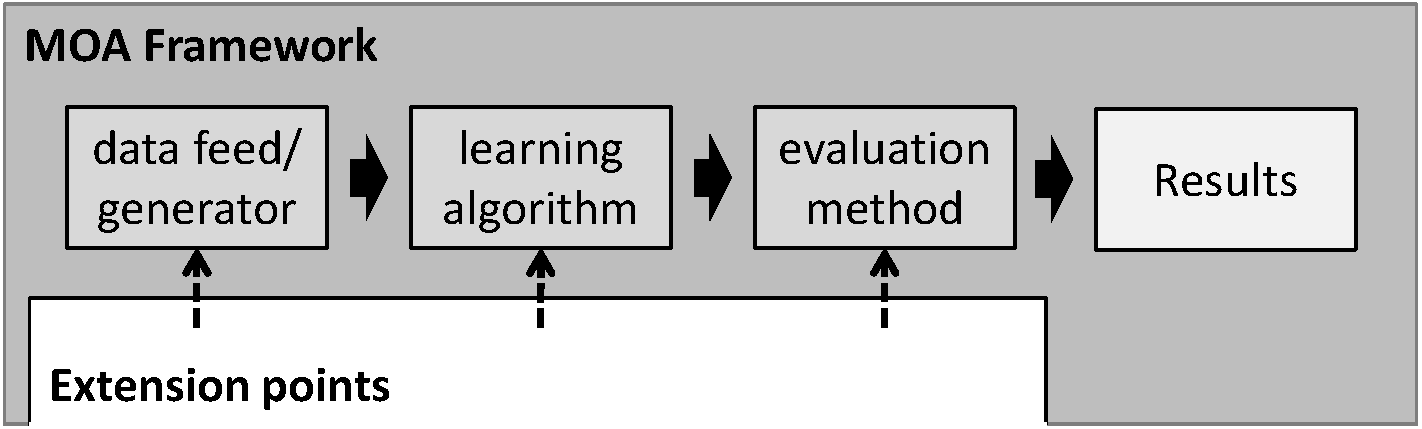
\includegraphics[scale=0.5]{frameworkGeneral.png}
	\end{figure}
	\note{MOA is an open-source framework software that allows to build and run experiments of machine learning or data mining on evolving data streams. }
\end{frame}

\begin{frame}
        \frametitle{Datasets}
        \begin{itemize}
        	\item twittersentiment.appspot.com
        	\begin{itemize}
        		\item :), :-), : ), :D, and =D - Positive
        		\item :(, :-(, and : ( - Negative
        		\item Training set - 800.000 positive and negative tweets
        		\item Test set - 182 positive, and 177 negative
        	\end{itemize}
        	\item Edinburgh corpus
        	\begin{itemize}
        		\item 97 million tweets
        		\item Feature reduction
	        	\begin{itemize}
	        		\item huuuuuungry $\rightarrow$ huungry
	        		\item @ $\rightarrow$ USER token
	        		\item URLs $\rightarrow$ URL token
	        	\end{itemize}
        		\item Used English tweets with emoticons
        		\begin{itemize}
        			\item Deleted after annotation
        		\end{itemize}
        		\item Reduced to a training set of 324,917 negative and 1,8m positive tweets
        	\end{itemize}
        \end{itemize}
\end{frame}